%\title{LaTeX Portrait Poster Template}
%%%%%%%%%%%%%%%%%%%%%%%%%%%%%%%%%%%%%%%%%
% a0poster Portrait Poster
% LaTeX Template
% Version 1.0 (22/06/13)
%
% The a0poster class was created by:
% Gerlinde Kettl and Matthias Weiser (tex@kettl.de)
% 
% This template has been downloaded from:
% http://www.LaTeXTemplates.com
%
% License:
% CC BY-NC-SA 3.0 (http://creativecommons.org/licenses/by-nc-sa/3.0/)
%
%%%%%%%%%%%%%%%%%%%%%%%%%%%%%%%%%%%%%%%%%

%----------------------------------------------------------------------------------------
%	PACKAGES AND OTHER DOCUMENT CONFIGURATIONS
%----------------------------------------------------------------------------------------

\documentclass[a0,portrait]{a0poster}

\usepackage{graphicx}
\usepackage{multicol} % This is so we can have multiple columns of text side-by-side
\columnsep=100pt % This is the amount of white space between the columns in the poster
\columnseprule=3pt % This is the thickness of the black line between the columns in the poster

%\usepackage[svgnames]{xcolor} % Specify colors by their 'svgnames', for a full list of all colors available see here: http://www.latextemplates.com/svgnames-colors

\usepackage{times} % Use the times font
%\usepackage{palatino} % Uncomment to use the Palatino font

\usepackage{graphicx} % Required for including images
\graphicspath{{figures/}} % Location of the graphics files
\usepackage{booktabs} % Top and bottom rules for table
\usepackage[font=normal,labelfont=bf]{caption} % Required for specifying captions to tables and figures
\usepackage{amsfonts, amsmath, amsthm, amssymb} % For math fonts, symbols and environments
\usepackage{wrapfig} % Allows wrapping text around tables and figures

\usepackage{hyperref}
\usepackage{xcolor}
\definecolor{DB}{RGB}{51,102,153}

\usepackage{tikz}
\usetikzlibrary{shapes,arrows,positioning,fit,backgrounds, arrows.meta}

\begin{document}

%----------------------------------------------------------------------------------------
%	POSTER HEADER 
%----------------------------------------------------------------------------------------

% The header is divided into two boxes:
% The first is 75% wide and houses the title, subtitle, names, university/organization and contact information
% The second is 25% wide and houses a logo for your university/organization or a photo of you
% The widths of these boxes can be easily edited to accommodate your content as you see fit

\begin{minipage}[b]{0.70\linewidth}
\veryHuge \color{DB} \textbf{A  Study  on  Brazilian  Portuguese  Verbal\\  Irregularities  via  Artificial  Neural  Networks } \color{black} \vspace{1cm}
\\ % Title
%\Huge\textit{An Exploration of Complexity}\\[2cm] % Subtitle
\huge \textbf{Beatriz Albiero}\\[0.5cm] % Author(s)
\huge University of Sao Paulo \\[0.4cm] % University/organization
\Large \texttt{beatriz.albiero@usp.br}\\
\end{minipage}
%
\begin{minipage}[b]{0.12\linewidth}
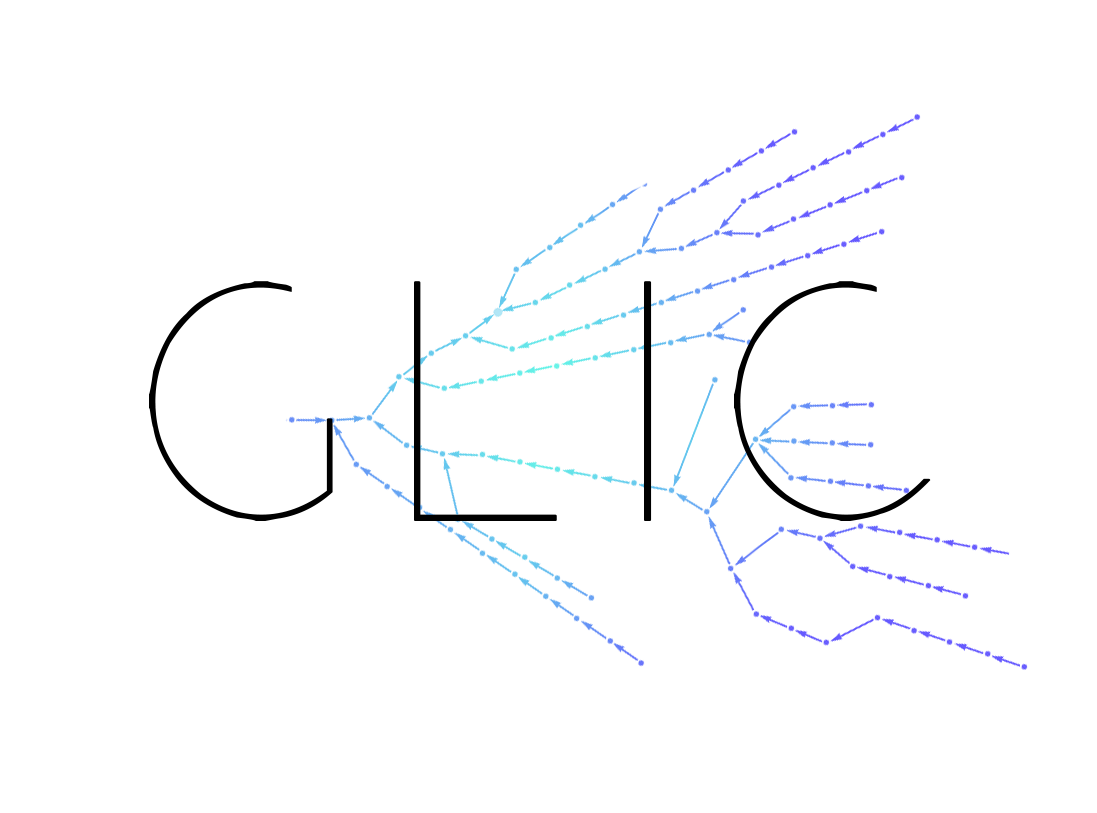
\includegraphics[width=1.4\textwidth]{Glic_Transparente.png}\\
\end{minipage}
\hspace{3cm}
\begin{minipage}[b]{0.12\linewidth}

\includegraphics[width=\textwidth]{DataLab-Logo-Alta.png}\\
\end{minipage}

\vspace{3.5cm} % A bit of extra whitespace between the header and poster content

%----------------------------------------------------------------------------------------

\begin{multicols}{2} % This is how many columns your poster will be broken into, a portrait poster is generally split into 2 columns

%----------------------------------------------------------------------------------------
%	ABSTRACT
%----------------------------------------------------------------------------------------

\color{DB} % Navy color for the abstract

\section*{Abstract}
\normalsize{ \color{darkgray}
 This project is an attempt at reproducing Rumelhart and McClelland's \cite{rumelhart:1986} connectionist experiment described in the book Parallel Distributed Processing, chapter "On learning the past tense of English verbs", with Brazilian Portuguese as a target language. In this book, Rumelhart and McClelland describe a new theory of cognition called connectionism that is challenging the idea of symbolic computation that has traditionally been at the center of the debate in theoretical discussions about the mind. In the chapter "On learning the past tense of English verbs", Rumelhart and McClelland describe an experiment in which a feedforward neural network was developed in order to find patterns among phonological features between present and past tense forms of English verbs. In this research, an identical network has been built to predict Brazilian Portuguese irregularities. We will discuss our model's results and the difficulties in adapting this model in order to predict irregularities in Brazilian Portuguese.
}

%----------------------------------------------------------------------------------------
%	INTRODUCTION
%----------------------------------------------------------------------------------------

\color{DB} % SaddleBrown color for the introduction

\section*{Introduction}
\normalsize{ \color{darkgray}
The process of verbal inflection from present to past tense in the English language is certainly one of the most controversial topics of debate among the main theoretical currents in linguistic study \cite{chomsky:1968,Pinker:1988,rumelhart:1986}.  At the heart of the debate is the exact characterization of the mechanisms that enable a speaker to relate a verb in present tense to its past tense form. 

The past tense of English is made up of a set of inflection families, which are split into two macro families: regular and irregular. Each macro family features subsets, grouped together by inflective similarity, with a noteworthy variety of families within the irregular group. This peculiar quality has motivated researchers D. Rumelhart and J. McClelland to build an artificial neural network model capable of predicting said inflective processes. While it is also possible to observe inflective regularities within irregular verb families in Brazilian Portuguese, the question remains: is it possible to adapt Rumelhart and McClelland's model to such language?   
}

%----------------------------------------------------------------------------------------
%	OBJECTIVES
%----------------------------------------------------------------------------------------

\color{DB} % DarkSlateGray color for the rest of the content

\section*{Main Objectives}

\color{darkgray}

\begin{itemize}
\item \large{The development of predictive computational  models (artificial neural networks) capable of detecting inflective phonological patterns within irregular verb families in Brazilian Portuguese.}
\item \large{Analysis of the model's results.}
\end{itemize} 
%----------------------------------------------------------------------------------------
%	MATERIALS AND METHODS
%----------------------------------------------------------------------------------------
\color{DB}
\section*{Methodology}
\color{darkgray}
A corpus of four hundred and three verbs, both in the infinitive and in the first person singular of the indicative, was built via web-scraping techniques. The material was then translated into a pseudo-phonological writing system, which was further codified into Wickelfeatures. A Feed Forward Neural Network was then built with the help of Keras library \cite{chollet2015keras}.
The network, similar to the one presented by the authors, is basically made up of two simple layers. The first layer is responsible for receiving the input data, which is a codified representation of the phonological features, the sounds, of a verb in the infinitive form (\textbf{Wickelfeatures})\cite{rumelhart:1986}. The second layer outputs identically codified phonological features, however, conjugated in the first person singular of the present tense. The first person singular was chosen by virtue of its moderate range of inflective variations. The results were then arranged into tables for further analysis. 

%------------------------------------------------

\color{DB}
\subsection*{Architecture}

\color{black}
\begin{center}
\definecolor{blue}{RGB}{159, 192, 176}
\definecolor{green}{RGB}{160, 227, 127}
\definecolor{orange}{RGB}{243, 188, 125}
\definecolor{red}{RGB}{253, 123, 84}
\definecolor{nephritis}{RGB}{39, 174, 96}
\definecolor{emerald}{RGB}{46, 204, 113}
\definecolor{turquoise}{RGB}{39, 174, 96}
\definecolor{green-sea}{RGB}{22, 160, 133}
\definecolor{purple}{RGB}{181, 124, 215}
% Tikzstyles for Computation Graphs

% nodes
\tikzstyle{noop} = [circle, draw=none, fill=red, minimum size = 10pt]
\tikzstyle{op} = [circle, draw=red, line width=1.5pt, fill=red!70, text=black, text centered, font=\bf \normalsize, minimum size = 25pt]

\tikzstyle{opintense} = [circle, draw=red, line width=1.5pt, fill=red!150, text=black, text centered, font=\bf \normalsize, minimum size = 25pt]


%new style
\tikzstyle{gp} = [circle, draw=red, line width=4pt, text=black, text centered, font=\bf \normalsize, minimum size = 4.cm]

\tikzstyle{box} = [rectangle, draw=red, line width=1.5pt, fill=red!70, text=black, align=center, font=\bf \normalsize, minimum size = 45pt]

\tikzstyle{state} = [circle, draw=blue, line width=1.5pt, fill=blue!70, text=black, text centered, font=\bf \normalsize, minimum size = 25pt]

\tikzstyle{output} = [circle, draw=purple, line width=1.5pt, fill=purple!70, text=black, text centered, font=\bf \normalsize, minimum size = 25pt]


\tikzstyle{gradient} = [circle, draw=nephritis, line width=1.5pt, fill=nephritis!60, text=black, text centered, font=\bf \normalsize, minimum size = 25pt]
\tikzstyle{textonly} = [draw=none, fill=none, text centered, font=\bf \normalsize]
\tikzstyle{boxtextonly} = [draw=none, fill=none, align=center, font=\bf \normalsize]

\tikzstyle{normal} = [circle, draw=black, line width=1.0pt, fill=none, text=black, text centered, font=\bf \normalsize, minimum size = 20pt]


% edges
\tikzstyle{tedge}  = [draw, thick, >=latex, ->]
\tikzstyle{tedge_dashed}  = [draw, thick, >=latex, ->, dashed]
\tikzstyle{nedge}  = [draw, thick, >=latex]
\tikzstyle{nedge_dashed}  = [draw, thick, >=latex, dashed]


% namedscope
\tikzstyle{namedscope} = [circle, draw=orange, line width=1.5pt, fill=orange!60, align=center, inner sep=0pt]
% \begin{figure}[]
% \centering

\scalebox{1.5}{

\begin{tikzpicture}[auto]
\centering
% operations =========
% phon features 1
\node[textonly] (1pho1) {[high, vowel, front]};

% Legenda
\node[textonly, above=10pt of 1pho1] (leg1) {Input Units};


% FNN input
\node[normal, right=5pt of 1pho1] (x1) {};
\node[normal, below=25pt of x1] (x2) {};
\node[normal, below=25pt of x2] (x3) {};
\node[normal, below=25pt of x3] (x4) {};
\node[normal, below=25pt of x4] (x5) {};
\node[normal, below=25pt of x5] (x6) {};

% FNN output
\node[normal, right=85pt of x1] (y1) {};
\node[normal, right=85pt of x2] (y2) {};
\node[normal, right=85pt of x3] (y3) {};
\node[normal, right=85pt of x4] (y4) {};
\node[normal, right=85pt of x5] (y5) {};
\node[normal, right=85pt of x6] (y6) {};

% phon features 2
\node[textonly, right=5pt of y1] (2pho1) {[high, vowel, front]};
\node[textonly, above=10pt of 2pho1] (leg2) {Output Units};
\node[textonly, left=25pt of x2] (1pho2) {[low, back, nasal]};
\node[textonly, right=25pt of y2] (2pho2) {[low, back, nasal]};
\node[textonly, left=25pt of x3] (3pho1) {...};
\node[textonly, right=25pt of y3] (1pho3) {...};
\node[textonly, left=25pt of x6] (6pho1) {[vowel, nasal, middle]};
\node[textonly, right=25pt of y6] (1pho6) {[vowel, nasal, middle]};
% edges FNN
\path[nedge] (x1) -- (y1);
\path[nedge] (x1) -- (y2);
\path[nedge] (x1) -- (y3);
\path[nedge] (x1) -- (y4);
\path[nedge] (x1) -- (y5);
\path[nedge] (x1) -- (y6);
\path[nedge] (x2) -- (y1);
\path[nedge] (x2) -- (y2);
\path[nedge] (x2) -- (y3);
\path[nedge] (x2) -- (y4);
\path[nedge] (x2) -- (y5);
\path[nedge] (x2) -- (y6);
\path[nedge] (x3) -- (y1);
\path[nedge] (x3) -- (y2);
\path[nedge] (x3) -- (y3);
\path[nedge] (x3) -- (y4);
\path[nedge] (x3) -- (y5);
\path[nedge] (x3) -- (y6);
\path[nedge] (x4) -- (y1);
\path[nedge] (x4) -- (y2);
\path[nedge] (x4) -- (y3);
\path[nedge] (x4) -- (y4);
\path[nedge] (x4) -- (y5);
\path[nedge] (x4) -- (y6);
\path[nedge] (x5) -- (y1);
\path[nedge] (x5) -- (y2);
\path[nedge] (x5) -- (y3);
\path[nedge] (x5) -- (y4);
\path[nedge] (x5) -- (y5);
\path[nedge] (x5) -- (y6);
\path[nedge] (x6) -- (y1);
\path[nedge] (x6) -- (y2);
\path[nedge] (x6) -- (y3);
\path[nedge] (x6) -- (y4);
\path[nedge] (x6) -- (y5);
\path[nedge] (x6) -- (y6);


\end{tikzpicture}
}
% }\caption{Neural Net Scheme} 
% \label{fig:esquemafdd}
% \end{figure}
\captionof{figure}{Neural Artificial Network Scheme}
\end{center}
\color{DB}
\subsection*{Corpus}
\color{darkgray}
403 verbs, divided into two parts: test ($\thicksim$20\%) and training ($\thicksim$80\%)\vspace{1cm}

\begin{center}
\begin{minipage}{0.45\textwidth}\centering
\begin{tabular}{lllll}
\hline
 & \textbf{Regulars} & \textbf{Irregulars} & \textbf{Total} & \textbf{\%} \\ \hline
\textbf{Test} & 42 & 36 & 78 & 19.35 \\ \hline
\textbf{Train} & 172 & 153 & 325 & 80.65 \\ \hline
\textbf{Total} & 214 & 189 & 403 & 100 \\ \hline
\end{tabular}
\captionof{table}{Regular-irregular ratios in datasets}
\label{tab1}
\end{minipage}
\end{center}




%----------------------------------------------------------------------------------------
%	RESULTS 
%----------------------------------------------------------------------------------------
\color{DB}
\section*{Results}
\color{darkgray}
	A small set of 21 verbs was used to test the accuracy of the model. Since all verbs in the infinitive form end in the phoneme “r”, the deletion of this phoneme reduced redundancies and facilitated the decoding of wickelfeatures. In order to test the relevance of the irregular verb ratio for the model’s accuracy, five datasets, each with a different regular-irregular verb ratio, were tested, with the best infinitive to first person singular prediction accuracy being 47.62\% for two sets: one made up of 55\% irregular verbs and other made up of 95\% irregular verbs.

Verbs exceeding four phonemes did not yield satisfactory Wickelfeature to Pseudo-Phonological-Writing decoding results.

\begin{center}\vspace{1cm}
\begin{minipage}[b]{0.45\linewidth}\centering
\begin{tabular}{llll}
\textbf{Ratio} & \textbf{Epochs} & \textbf{Batch Size} & \textbf{Accuracy} \\
\toprule
55\% & 400 & 464 & 47.62\% \\
65\% & 400 & 565 & 38.10\% \\
75\% & 400 & 388 & 38.10\% \\
85\% & 400 & 390 & 42.86\% \\
95\% & 400 & 395 & 47.62\%
\end{tabular}
\captionof{table}{Accuracy results for different ratios of irregular verbs.}
\end{minipage}
\hspace{0.5cm}
\begin{minipage}[b]{0.45\linewidth}
\centering
\begin{tabular}{llll}
\textbf{Verb} & \textbf{Input} & \textbf{Expected} & \textbf{Output} \\ \hline
pegar & \#pega\# & \#pEgu\# & \#pEku\# \\
cegar & \#sega\# & \#sEgu\# & \#sigu\# \\
secar & \#seka\# & \#sEku\# & \#siku\# \\
levar & \#leva\# & \#lEvu\# & \#levu\# \\
orar & \#ora\# & \#Oru\# & \#earu\# \\
morar & \#mora\# & \#mOru\# & \#mEru\# \\
postar & \#posta\# & \#pOstu\# & \#pOtu\#* \\
mentir & \#menti\# & \#mintu\# & \#mitu\#* \\
tossir & \#tosi\# & \#tusu\# & \#tutu\# \\
fazer & \#faze\# & \#fasu\# & \#fasu\# \\
matar & \#mata\# & \#matu\# & \#matu\# \\
pagar & \#paga\# & \#pagu\# & \#pagu\# \\
\#sair\# & \#sai\# & \#saiu\# & \#saiu\#
\end{tabular}
\captionof{table}{Some outputs of the model}
\end{minipage}
\end{center}


%----------------------------------------------------------------------------------------
%	CONCLUSIONS
%----------------------------------------------------------------------------------------

\color{DB} % SaddleBrown color for the conclusions to make them stand out

\section*{Conclusions}

\begin{itemize}
\color{darkgray}
\item \large Changing the ratio of irregular verbs in the training set apparently did not cause significant changes in accuracy, as shown in Table 2. It happened probably because the training dataset was made up of a small variety of verbs and enlarging its irregular verb classes simply resulted in the strengthening of connections for the Wickelfeatures that it already knew, culminating in a poor generalization capacity.
\item  \large The process of decoding Wickelfeatures into the pseudo-phonological writing system failed to yield satisfactory outcomes due to excessive binding redundancy within the Feed Forward Neural Network. The inadequacy of such model called for the implementation of a new strategy, which led to further research into Recurrent Neural Networks, particularly, the Encoder-Decoder technique. 
\end{itemize}

\color{darkgray} % Set the color back to DarkSlateGray for the rest of the content

%----------------------------------------------------------------------------------------
%	FORTHCOMING RESEARCH
%----------------------------------------------------------------------------------------
\color{DB}
\section*{Forthcoming Research}

\begin{itemize}
\color{darkgray}
\item \large Encoder-Decoder Model implementation with the purpose of better decoding Wickelfeatures.
\item \large Once the decoding of Wickelfeatures is properly contrived, a psycho-linguistic test will take place, in order to measure native speaker intuition against the Neural Network output.
\end{itemize}
 %----------------------------------------------------------------------------------------
%	REFERENCES
%----------------------------------------------------------------------------------------

\color{DB}
\nocite{*} % Print all references regardless of whether they were cited in the poster or not
\bibliographystyle{plain} % Plain referencing style
\bibliography{sample} % Use the example bibliography file sample.bib

%----------------------------------------------------------------------------------------
%	ACKNOWLEDGEMENTS
%----------------------------------------------------------------------------------------
\color{DB}
\section*{Acknowledgements}
\color{darkgray}
I would like to express my very great appreciation to Marcelo Barra, Livy Real, Romulo Ferreira, the DataLab team, NAACL Emerging Regions Fund and the Linguistics Graduation Department (FFLCH-USP).

%----------------------------------------------------------------------------------------

\end{multicols}
\end{document}